% =====================================================================
%  NEW TEXT FOR CHAPTER 2 (SoLD)
%  Generated from analyses in scripts/chapter2_addons/
%  See PLACEMENT_GUIDE.md for where each block goes.
% =====================================================================


% =====================================================================
% BLOCK 1 — RESULTS
% INSERT AFTER the subsection "Lipid variation across genotypes",
% BEFORE "Lipidome overview for CTL and LIN SAP".
% =====================================================================

\subsection{Lipid variation is largely independent of botanical race and population structure}

Because the SAP is strongly structured by botanical race and by geographic origin \citep{Casa2008, Boatwright2022}, we next asked whether the lipid variation described above simply tracks that structure. Two complementary groupings were tested. The first was botanical race, taken from the SAP passport data and collapsed into six groups: the five classical races (Bicolor, Caudatum, Durra, Guinea, Kafir) and a combined Mixed group containing all intermediate designations (e.g. Durra--Bicolor, Kafir--Caudatum). Race information was available for 222 of 394 CTL accessions and 211 of 363 LIN accessions, with group sizes of 17/16 (Bicolor), 76/71 (Caudatum), 22/23 (Durra), 19/17 (Guinea), 7/7 (Kafir) and 81/77 (Mixed) in CTL/LIN respectively. The second grouping was the marker-based genetic cluster assignment ($K=6$), which covered 387 CTL and 355 LIN accessions and therefore provides a more complete and more directly genetic description of population structure. For each grouping we tested 14 traits per condition -- total lipid signal (log$_{10}$ TIC) and the 13 major class \%TIC values -- using Kruskal--Wallis tests with Benjamini--Hochberg correction applied within condition, and summarised effect size as $\varepsilon^2$, the proportion of rank variance attributable to the grouping.

Botanical race explained essentially none of the lipid variation. No trait was significant in either condition after BH correction; the smallest raw $p$-values were $p=0.0397$ for PG in LIN ($q=0.468$) and $p=0.0648$ for TG in CTL ($q=0.492$). Effect sizes were correspondingly small, with $\varepsilon^2$ ranging from $0$ to $0.033$ across all traits and both conditions (Table~\ref{tab:race_structure}, Fig.~\ref{fig:race_structure}). The genetic-cluster analysis gave the same result for 13 of the 14 traits, with $q>0.20$ and $\varepsilon^2<0.021$ throughout. The single exception was phosphatidylserine under LIN, where genetic cluster was strongly associated with PS abundance ($H=43.43$; $p=3.02\times10^{-8}$; $q=4.23\times10^{-7}$; $\varepsilon^2=0.110$). The same trait showed a weaker and non-significant trend under CTL ($q=0.206$; $\varepsilon^2=0.024$), indicating that the association is not a stable property of the trait across trials.

These results have two consequences for the interpretation of the GWAS reported below. First, because neither race nor genome-wide cluster assignment accounts for more than a few percent of the variance in any lipid class, the association signals we report are unlikely to be straightforward artefacts of population stratification, and the three genotype principal components included in the mixed model are adequate for these traits. Second, PS is a documented exception and should be treated more cautiously than the other classes: it is the only trait whose abundance is appreciably structured by genetic cluster in one of the two trials, and it is also present at very low relative abundance (mean $0.014\%$ of TIC in CTL and $0.037\%$ in LIN, compared with $34.5\%$ and $32.1\%$ for MGDG). The PS contrast is therefore reproducible in direction and detected without missing values, but it describes a redistribution within a minor pool rather than a large shift in the bulk lipidome.

\begin{table*}[!ht]
\centering
\caption{\textbf{Population structure explains little lipid-class variation.} Effect sizes ($\varepsilon^2$, proportion of rank variance explained) from Kruskal--Wallis tests of each trait against botanical race (six groups) and marker-based genetic cluster ($K=6$), computed separately within each field trial. $\varepsilon^2$ was truncated at zero. Significance is after Benjamini--Hochberg correction within condition: *** $q<0.001$; all other entries $q>0.20$.}
\label{tab:race_structure}
\small
\begin{tabular}{lcccc}
\toprule
& \multicolumn{2}{c}{\textbf{Botanical race}} & \multicolumn{2}{c}{\textbf{Genetic cluster ($K=6$)}} \\
\cmidrule(lr){2-3}\cmidrule(lr){4-5}
\textbf{Trait} & \textbf{CTL} & \textbf{LIN} & \textbf{CTL} & \textbf{LIN} \\
\midrule
Total lipid (log$_{10}$ TIC) & 0.000 & 0.020 & 0.000 & 0.000 \\
MGDG & 0.000 & 0.014 & 0.000 & 0.000 \\
PC   & 0.000 & 0.006 & 0.002 & 0.000 \\
DG   & 0.000 & 0.003 & 0.002 & 0.007 \\
DGDG & 0.000 & 0.014 & 0.000 & 0.000 \\
TG   & 0.025 & 0.000 & 0.010 & 0.013 \\
PE   & 0.020 & 0.000 & 0.007 & 0.021 \\
SQDG & 0.000 & 0.024 & 0.000 & 0.013 \\
MG   & 0.017 & 0.000 & 0.005 & 0.012 \\
PG   & 0.009 & 0.033 & 0.000 & 0.004 \\
PA   & 0.015 & 0.000 & 0.000 & 0.005 \\
LPC  & 0.008 & 0.000 & 0.003 & 0.004 \\
PS   & 0.000 & 0.002 & 0.024 & \textbf{0.110}*** \\
LPE  & 0.000 & 0.000 & 0.001 & 0.000 \\
\midrule
\textbf{$n$ accessions} & 222 & 211 & 387 & 355 \\
\bottomrule
\end{tabular}
\end{table*}

\begin{figure*}[!ht]
\centering
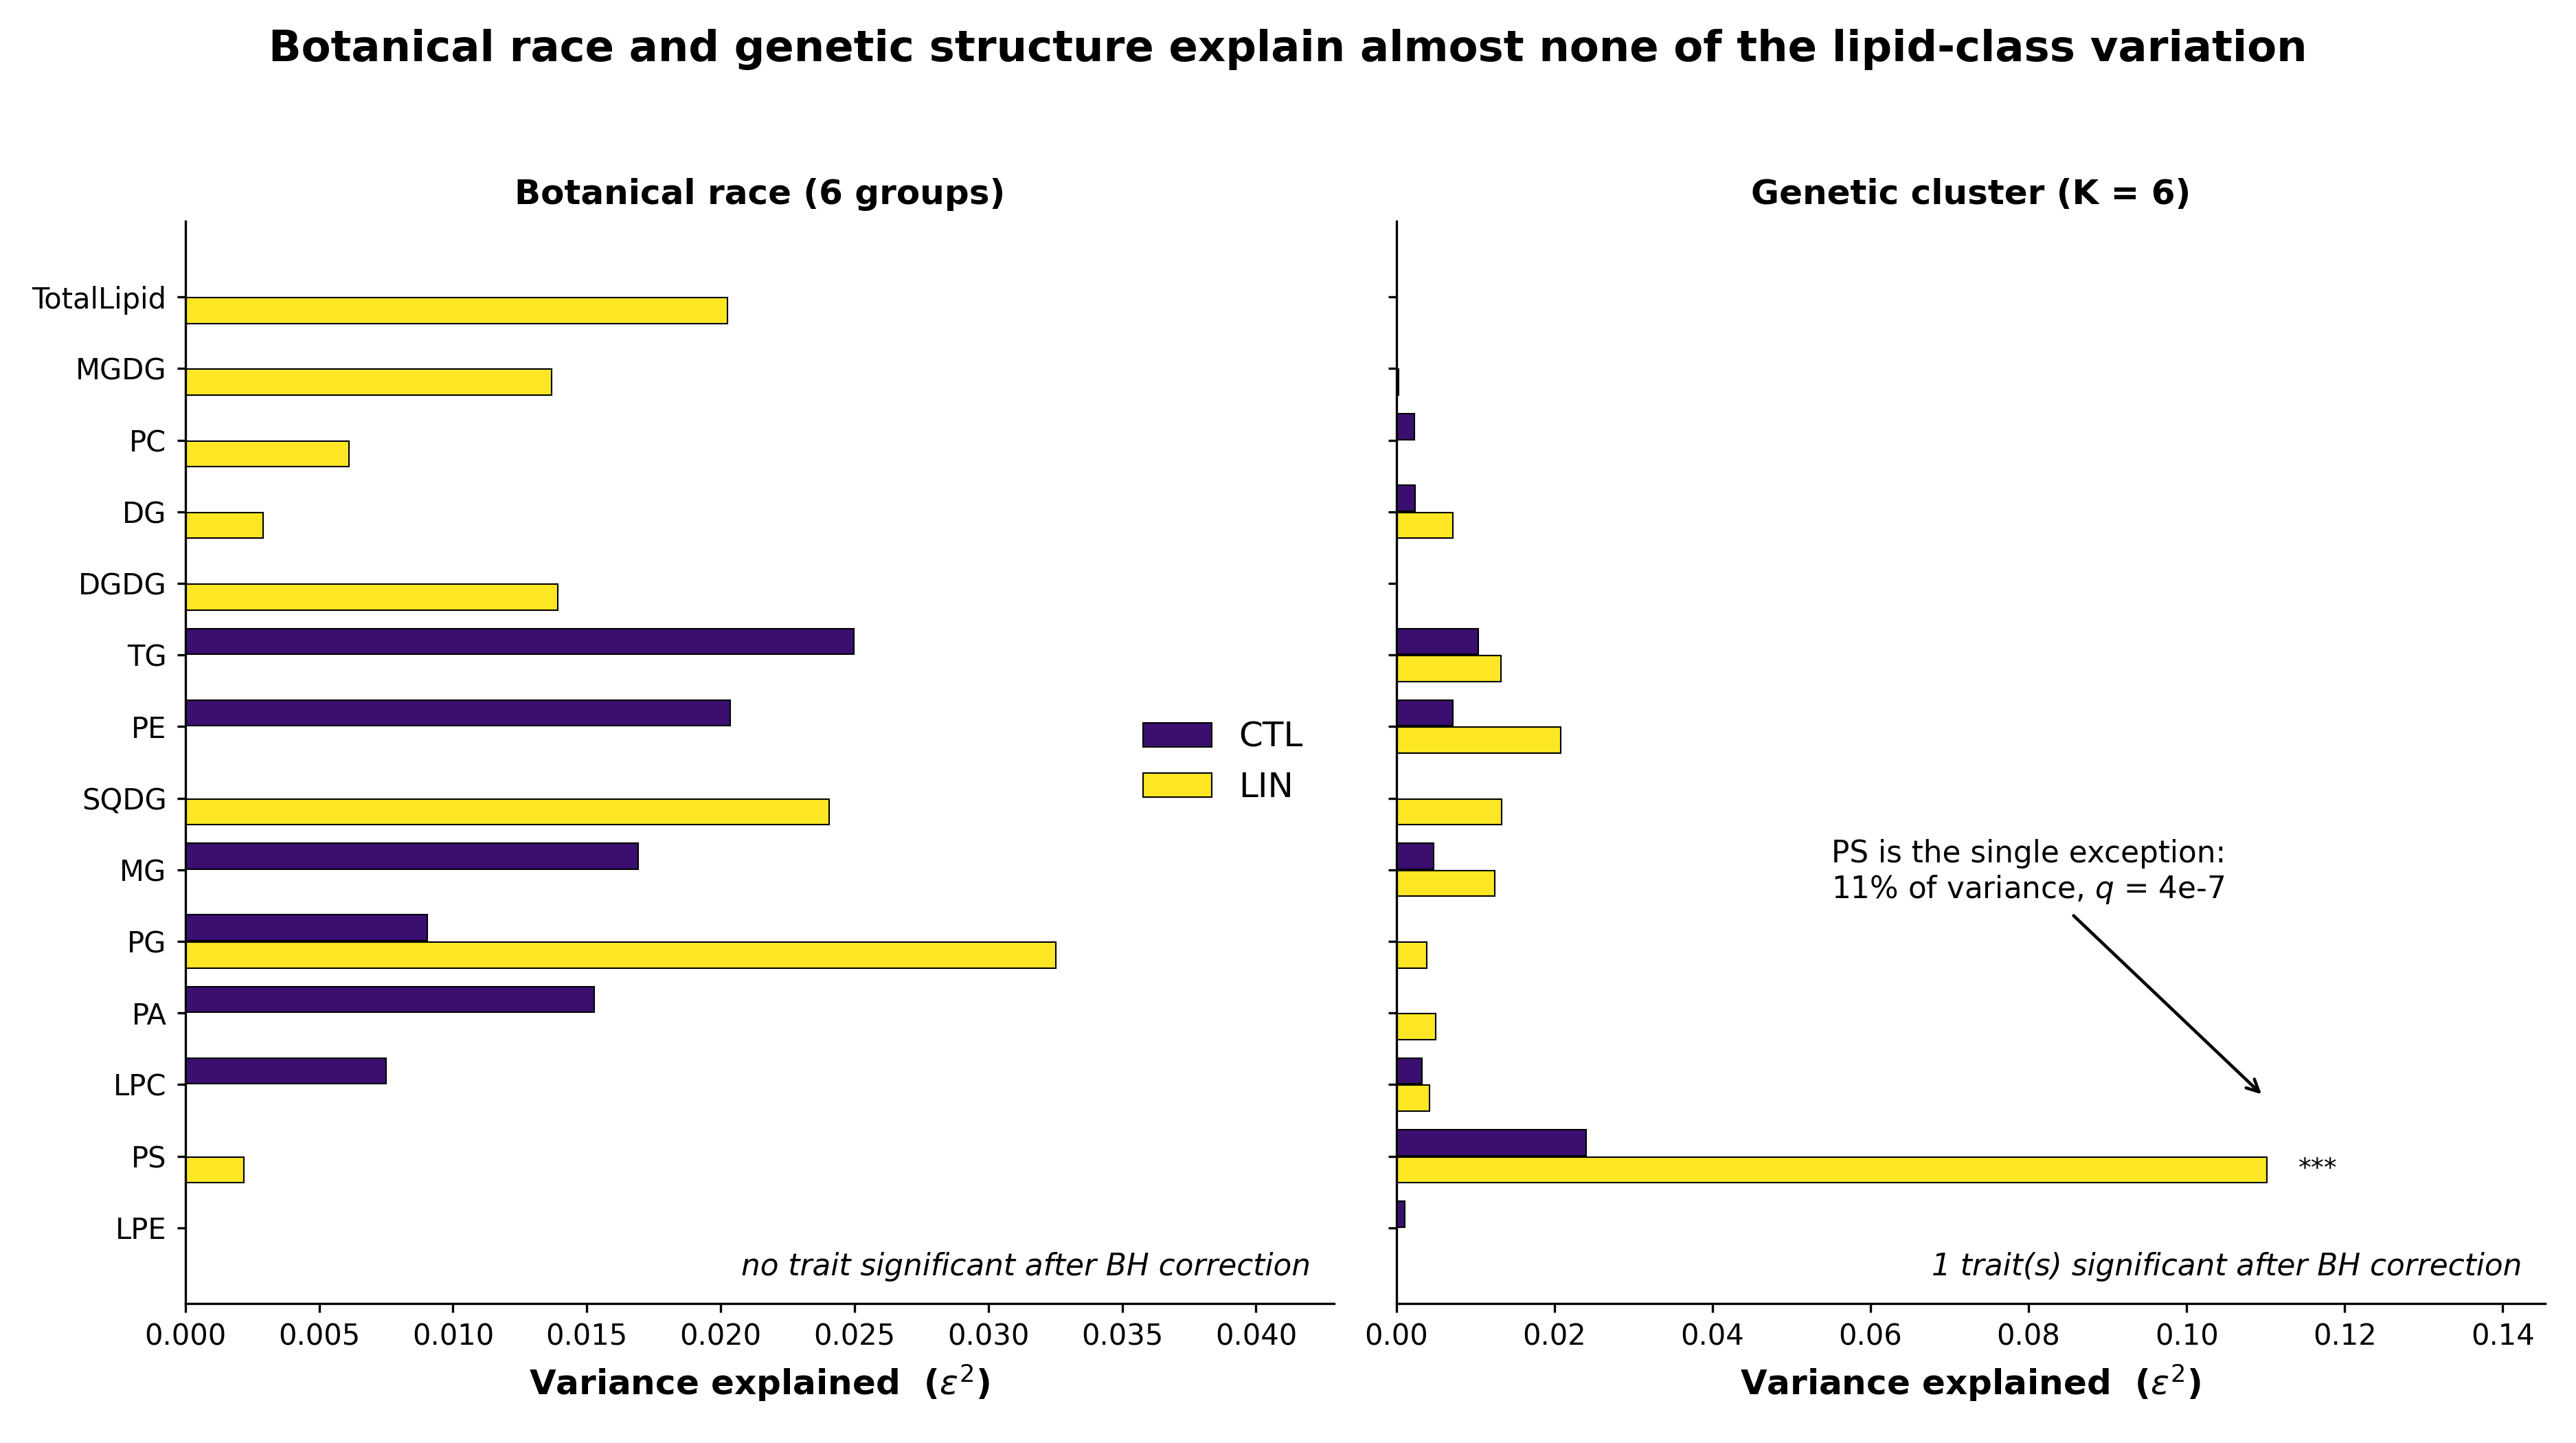
\includegraphics[width=\textwidth]{fig/race/FigRace_C_variance_explained.png}
\caption{\textbf{Botanical race and genetic structure explain almost none of the lipid-class variation.} Variance explained ($\varepsilon^2$) by botanical race (left) and by marker-based genetic cluster ($K=6$, right) for total lipid signal and 13 lipid classes, shown separately for CTL and LIN. No trait is significant by race in either condition after Benjamini--Hochberg correction. Phosphatidylserine under LIN is the single trait strongly associated with genetic cluster.}
\label{fig:race_structure}
\end{figure*}


% =====================================================================
% BLOCK 2 — RESULTS
% INSERT AFTER "LIN recurrent GWAS signals and annotation-based
% functional enrichment", BEFORE the LINEX subsection.
% =====================================================================

\subsection{CTL and LIN candidate loci overlap no more than expected by chance}

The CTL and LIN analyses above were run independently, and their functional enrichments differed. To test whether that difference is quantitative rather than impressionistic, we compared the two candidate sets directly. Overlap was assessed against a background of the 34{,}027 annotated \textit{Sorghum bicolor} v3.1 gene models using a hypergeometric test, and was summarised both as fold enrichment over chance and as the Jaccard index, which reports the fraction of the union that the two sets share.

At the level of individual genes the two sets appear to overlap strongly. Across all trait layers, 354 genes were recovered in both conditions against 148 expected by chance ($2.39\times$; $P=4.7\times10^{-59}$), and the effect was present in the individual-lipid layer alone (289 shared, $2.07\times$, $P=4.3\times10^{-35}$) and in the class-sum/ratio layer (18 shared, $6.56\times$, $P=2.9\times10^{-10}$). The Jaccard indices, however, were low throughout ($0.020$--$0.069$), indicating that although the shared fraction exceeds chance, it remains a small part of the combined candidate space.

This gene-level enrichment is largely an artefact of linkage disequilibrium. Because candidate genes are assigned to significant SNPs by LD, a single association recruits every gene model in the surrounding block, and gene-dense regions are recruited repeatedly in both trials. We therefore repeated the test after collapsing the genome into non-overlapping windows and counting a window as a hit if it contained at least one candidate gene (Table~\ref{tab:overlap}). At 100~kb resolution the individual-lipid enrichment fell to $1.15\times$ ($P=8.5\times10^{-3}$), and at 250~kb and 500~kb it was indistinguishable from chance ($1.04\times$, $P=0.23$; $1.03\times$, $P=0.29$). In other words, the loci recovered from the two trials are no more concordant than two independent samples of the same genome. The class-sum and class-ratio layer behaved differently: it retained a modest excess at 100~kb and 250~kb ($2.75\times$, $P=0.013$; $2.36\times$, $P=0.038$) before losing significance at 500~kb, indicating that composite class-level traits are somewhat more reproducible across trials than individual lipid species.

The same LD structure inflates the raw candidate counts. Collapsing to 250~kb loci, the 1{,}100 CTL and 4{,}323 LIN individual-lipid candidate genes correspond to 378 and 971 independent loci respectively, i.e. 2.9 and 4.5 gene models per locus (Table~\ref{tab:inflation}). Candidate-gene totals should therefore be read as an upper bound on the number of distinct signals.

Resolving the comparison by lipid class reinforces the same conclusion (Table~\ref{tab:overlap_class}). In the individual-lipid layer only TG and PC showed any significant excess, and both were weak (TG: 37 shared, $1.63\times$, $q=0.009$; PC: 8 shared, $3.55\times$, $q=0.009$). Free fatty acids showed no excess ($q=0.95$). SQDG, DG, AEG and terpenoids shared no candidate genes at all between the two trials, despite SQDG contributing 9 CTL and 396 LIN candidates. Moreover, sharing a gene did not usually mean sharing a phenotype: of the 354 genes recovered in both conditions, only 90 ($25.4\%$) were associated with at least one lipid class in common, falling to 52 of 289 ($18.0\%$) in the individual-lipid layer.

Finally, the small number of genuinely recurrent signals is concentrated in very few places in the genome. The 18 genes shared between conditions in the class-sum/ratio layer are not 18 independent loci but two contiguous LD blocks: a ten-gene block on chromosome~10 spanning \texttt{SORBI\_3010G150325}--\texttt{SORBI\_3010G151325}, which contains the CMP-sialic acid transporter \texttt{SORBI\_3010G151000} discussed above, and an eight-gene block on chromosome~1 spanning \texttt{SORBI\_3001G168800}--\texttt{SORBI\_3001G171600}. Together, these analyses show that the CTL and LIN lipid GWAS recover largely non-overlapping genetic architectures, that reported candidate-gene counts are inflated several-fold by LD, and that only a small number of loci -- concentrated in class-level composite traits -- recur across the two field trials.

\begin{table*}[!ht]
\centering
\caption{\textbf{Cross-trial overlap of GWAS candidates at gene and locus resolution.} Overlap between CTL and LIN candidate sets, tested against a background of 34{,}027 annotated gene models (gene level) or of all genome windows containing at least one gene (locus level). Fold, observed/expected shared; $J$, Jaccard index; $P$, hypergeometric (right-tail) test. Bold rows are the resolutions at which LD blocks are effectively collapsed.}
\label{tab:overlap}
\small
\begin{tabular}{llrrrrrrl}
\toprule
\textbf{Resolution} & \textbf{Trait layer} & \textbf{CTL} & \textbf{LIN} & \textbf{Shared} & \textbf{Exp.} & \textbf{Fold} & \textbf{$J$} & \textbf{$P$} \\
\midrule
Gene   & All layers          & 1165 & 4323 & 354 & 148.0 & 2.39 & 0.069 & $4.7\times10^{-59}$ \\
Gene   & Individual lipids   & 1100 & 4323 & 289 & 139.8 & 2.07 & 0.056 & $4.3\times10^{-35}$ \\
Gene   & Class sums / ratios &  115 &  812 &  18 &   2.7 & 6.56 & 0.020 & $2.9\times10^{-10}$ \\
\midrule
100 kb & Individual lipids   &  521 & 1564 & 193 & 168.2 & 1.15 & 0.102 & $8.5\times10^{-3}$ \\
100 kb & Class sums / ratios &   50 &  247 &   7 &   2.5 & 2.75 & 0.024 & $1.3\times10^{-2}$ \\
\textbf{250 kb} & \textbf{Individual lipids}   & 378 & 971 & 168 & 161.1 & \textbf{1.04} & 0.142 & \textbf{0.23} \\
250 kb & Class sums / ratios &   36 &  161 &   6 &   2.5 & 2.36 & 0.031 & $3.8\times10^{-2}$ \\
\textbf{500 kb} & \textbf{Individual lipids}   & 297 & 656 & 162 & 157.2 & \textbf{1.03} & 0.205 & \textbf{0.29} \\
500 kb & Class sums / ratios &   28 &  121 &   5 &   2.7 & 1.83 & 0.035 & 0.13 \\
\bottomrule
\end{tabular}
\end{table*}

\begin{table*}[!ht]
\centering
\caption{\textbf{LD inflates candidate-gene counts.} Candidate genes and the corresponding number of independent loci, defined as non-overlapping 250~kb genome windows containing at least one candidate gene.}
\label{tab:inflation}
\small
\begin{tabular}{llrrr}
\toprule
\textbf{Condition} & \textbf{Trait layer} & \textbf{Genes} & \textbf{Loci} & \textbf{Genes/locus} \\
\midrule
CTL & Individual lipids   & 1100 & 378 & 2.9 \\
CTL & Class sums / ratios &  115 &  36 & 3.2 \\
LIN & Individual lipids   & 4323 & 971 & 4.5 \\
LIN & Class sums / ratios &  812 & 161 & 5.0 \\
\bottomrule
\end{tabular}
\end{table*}

\begin{table*}[!ht]
\centering
\caption{\textbf{Per-class cross-trial overlap of individual-lipid GWAS candidates.} Genes were assigned to a lipid class through the phenotypes with which they were associated. $q$, Benjamini--Hochberg-adjusted hypergeometric $P$-value. n.s., not significant.}
\label{tab:overlap_class}
\small
\begin{tabular}{lrrrrl}
\toprule
\textbf{Class} & \textbf{CTL} & \textbf{LIN} & \textbf{Shared} & \textbf{Fold} & \textbf{$q$} \\
\midrule
TG          & 866 & 890 & 37 & 1.63 & $9.4\times10^{-3}$ \\
PC          &  58 & 1324 &  8 & 3.55 & $9.4\times10^{-3}$ \\
Fatty acid  & 109 & 1897 &  7 & 1.15 & 0.95 (n.s.) \\
Terpenoid   &  37 &  39 &  0 & --   & 1 (n.s.) \\
DG          &  13 &  34 &  0 & --   & 1 (n.s.) \\
SQDG        &   9 & 396 &  0 & --   & 1 (n.s.) \\
AEG         &   7 & 119 &  0 & --   & 1 (n.s.) \\
\bottomrule
\end{tabular}
\end{table*}

\begin{figure*}[!ht]
\centering
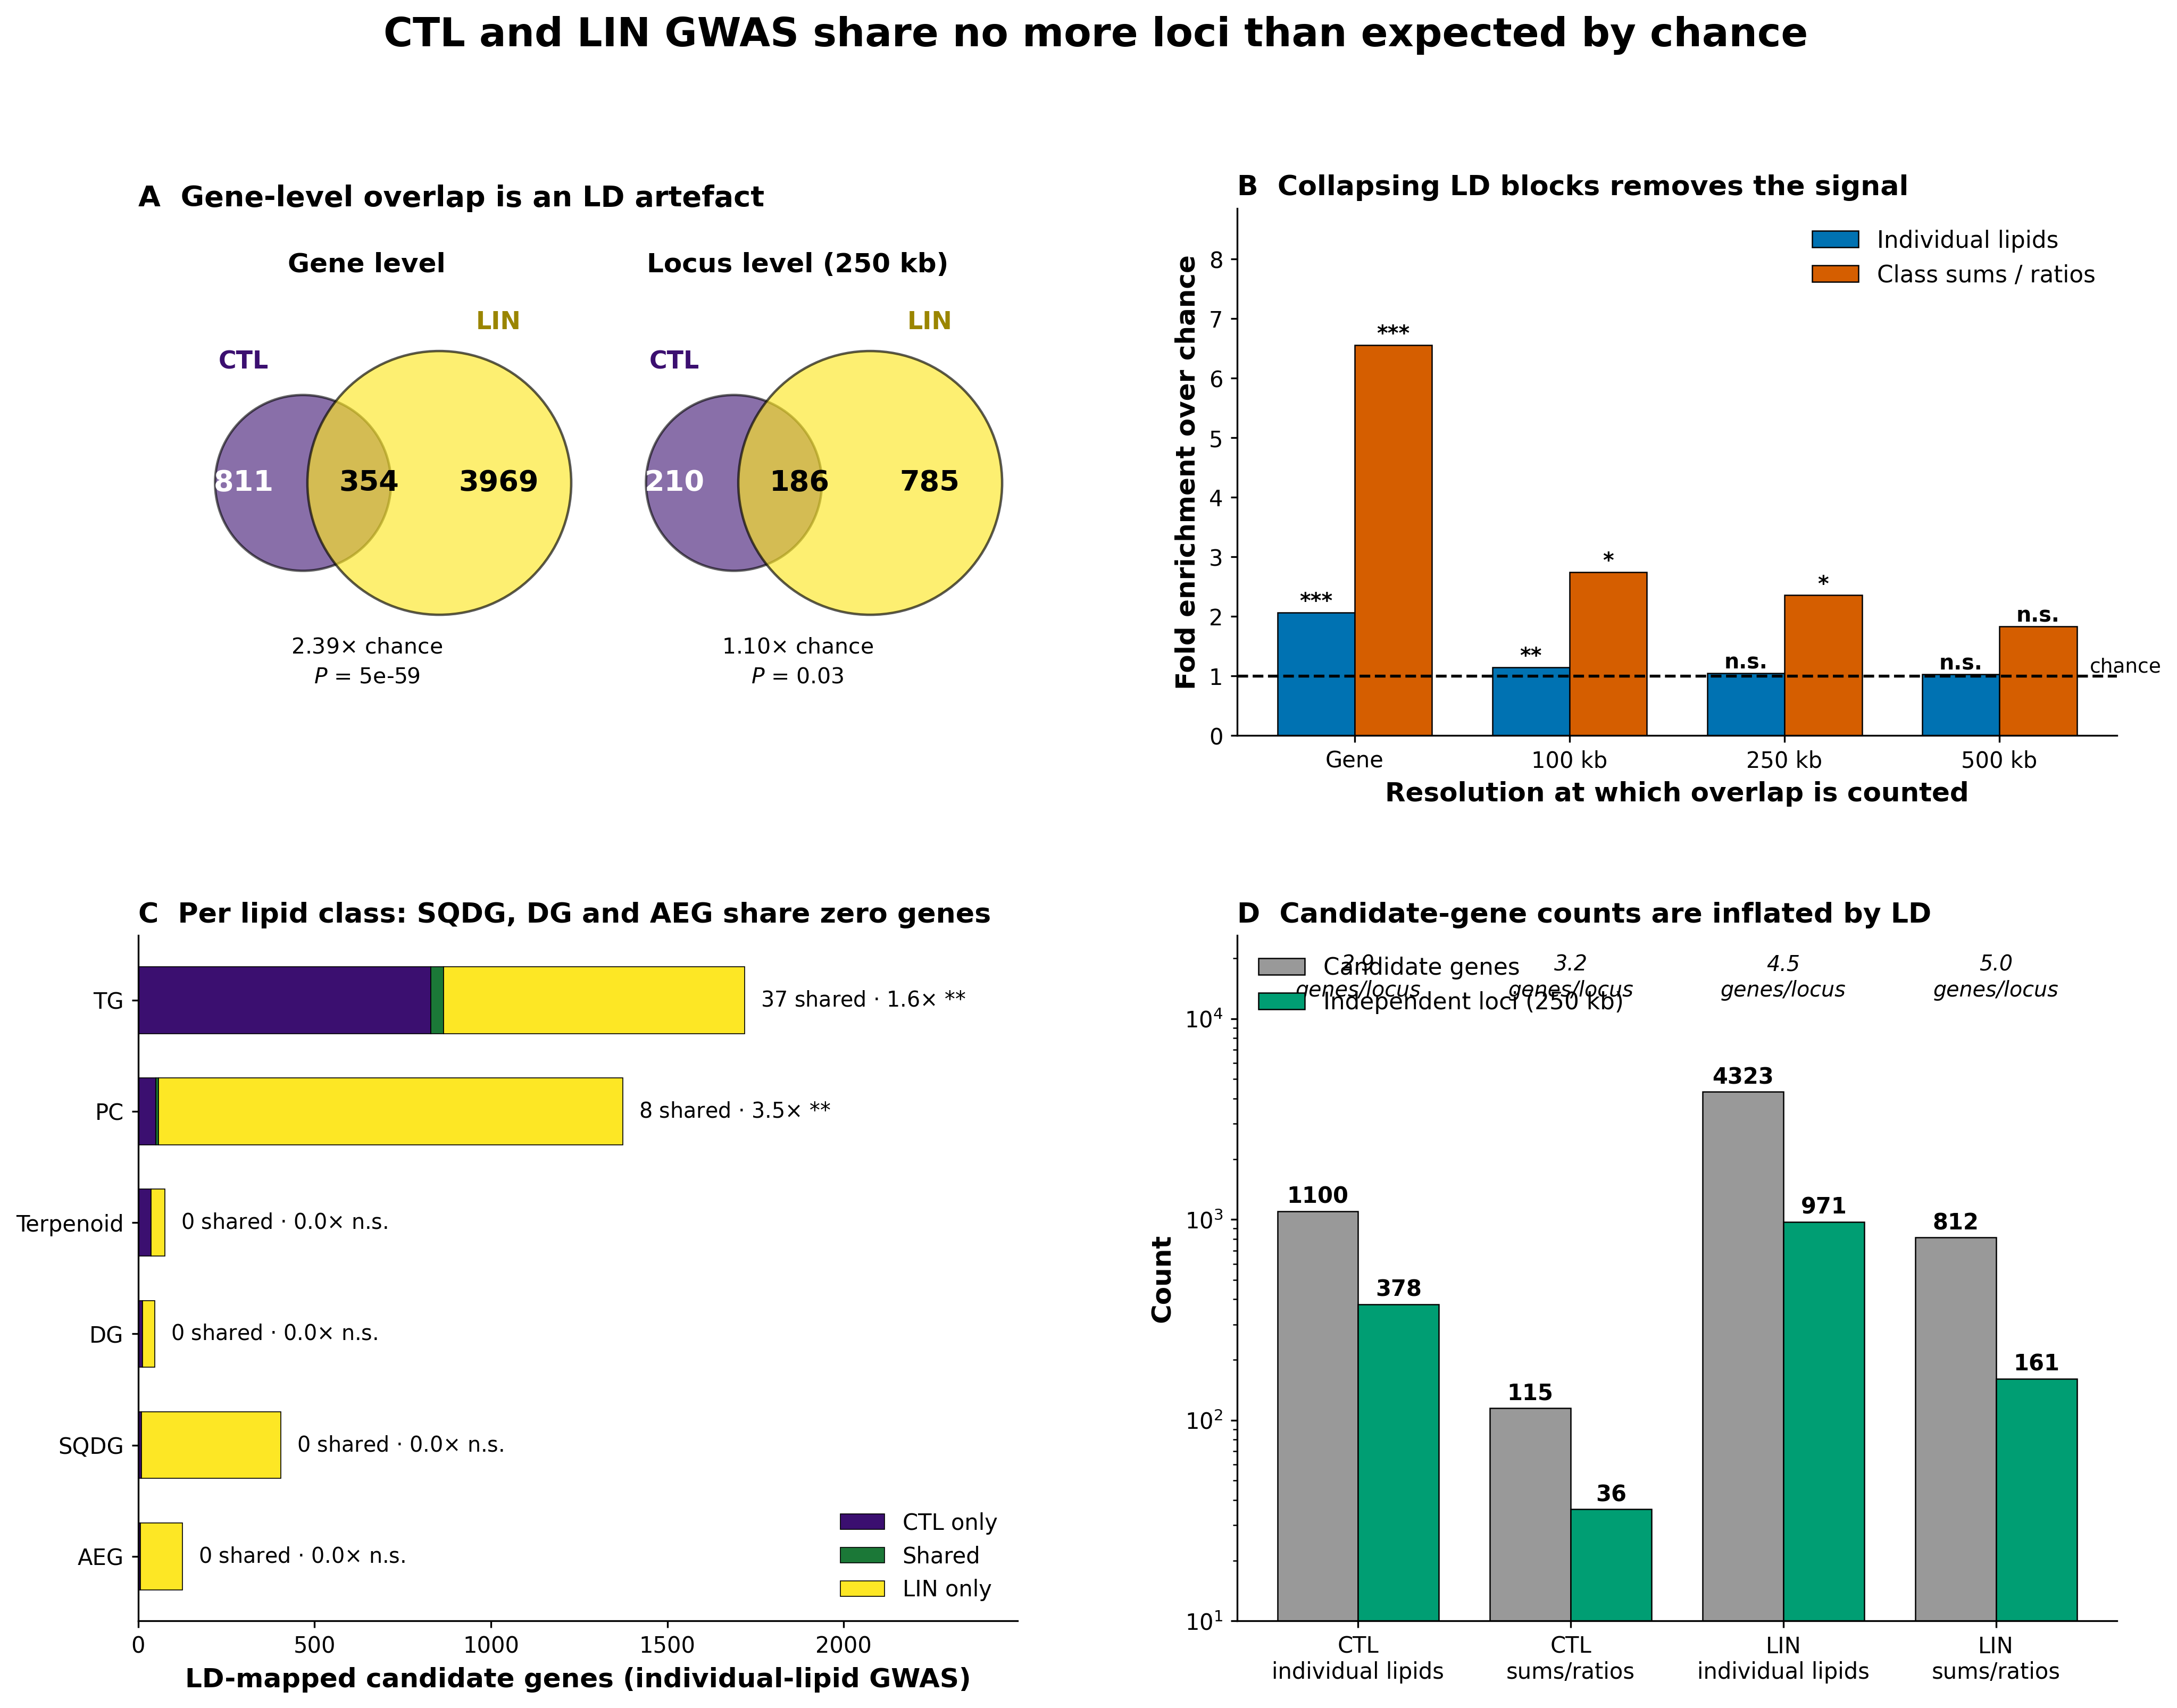
\includegraphics[width=\textwidth]{fig/overlap/FigOverlap_CTL_vs_LIN.png}
\caption{\textbf{CTL and LIN GWAS identify largely non-overlapping candidate loci.}
(A) Overlap of candidate sets at gene level and after collapsing linkage blocks into 250~kb loci, with fold enrichment over chance and hypergeometric $P$.
(B) Fold enrichment of the overlap as a function of the resolution at which it is counted, for individual-lipid and class-sum/ratio traits. The dashed line marks chance expectation; *** $P<0.001$, ** $P<0.01$, * $P<0.05$, n.s. not significant.
(C) Candidate genes per lipid class in the individual-lipid GWAS, partitioned into CTL-only, shared and LIN-only.
(D) Candidate-gene counts compared with the number of independent 250~kb loci they occupy (log scale).}
\label{fig:overlap}
\end{figure*}


% =====================================================================
% BLOCK 3 — DISCUSSION
% ADD as a new paragraph at the END of the subsection
% "Integrated interpretation of lipidome remodeling across contrasting
%  field trials".
% =====================================================================

Two of the four signatures also warrant an explicit statement of scale. PS and the lysophospholipids are minor components of the detected lipidome: PS accounted for a mean of $0.014\%$ of TIC under CTL and $0.037\%$ under LIN, and LPE for $0.006\%$ and $0.011\%$, against $34.5\%$ and $32.1\%$ for MGDG. These species were detected without missing values in every sample, so the contrasts are not detection artefacts, and their direction is consistent across analyses; but they describe redistribution within small pools rather than large changes in bulk membrane composition, and compositional transformations such as CLR necessarily amplify proportional changes in low-abundance components. PS carries a further caveat: it was the only trait whose abundance was appreciably associated with genome-wide genetic cluster, and only in LIN ($\varepsilon^2=0.110$; $q=4.2\times10^{-7}$). We therefore regard the PS and lysophospholipid signatures as robust in direction but modest in magnitude, and we place greater interpretive weight on the SQDG and TG axes, which involve classes contributing several percent of TIC.


% =====================================================================
% BLOCK 4 — DISCUSSION
% INSERT as a NEW subsection AFTER "Reaction-supported lipid-remodeling
% candidates under LIN implicate DG--TG cycling and phospholipid turnover".
% =====================================================================

\subsection{The genetic architecture of the sorghum leaf lipidome is strongly environment-dependent}

The candidate loci described in the two preceding sections were recovered from trials that differed in nutrient supply, planting date, management and year, and their functional enrichments diverged accordingly. The direct comparison of the two candidate sets makes the scale of that divergence explicit. Once linkage blocks are collapsed, the individual-lipid candidate loci recovered under CTL and under LIN overlap no more than two independent draws from the same genome ($1.04\times$ chance at 250~kb, $P=0.23$). Even among genes recovered in both trials, only $18\%$ were associated with a common lipid class, so the modest sharing that does exist is largely not trait-specific. The strong gene-level enrichment that is visible before collapsing LD blocks ($2.39\times$, $P=4.7\times10^{-59}$) is a property of how candidates are mapped rather than of the biology, and the same LD structure inflates candidate-gene totals by a factor of three to five. This has a practical implication for how such resources are read: counts such as the 4{,}323 LIN individual-lipid candidates correspond to roughly 971 independent loci, and comparisons between studies should be made at locus rather than gene resolution.

Two positive findings sit inside this largely negative result. First, class-level composite traits replicated better than individual species: class sums and class ratios retained a significant cross-trial excess at 100~kb and 250~kb resolution, where individual lipids did not. Aggregating species into class totals reduces the measurement noise carried by individual features and averages over the acyl-chain heterogeneity within a class, so composite traits are the more sensible unit for cross-environment comparison, and are also the level at which the lipidome-wide remodeling signatures were defined. Second, the loci that do recur are concentrated in two chromosomal regions, one of which contains the CMP-sialic acid transporter \texttt{SORBI\_3010G151000} that was independently among the most recurrent LIN candidates. Loci of this kind, recovered in both trials and across many class-level traits, are the most defensible starting points for validation.

We interpret this pattern as evidence that the genetic control of leaf lipid composition in the SAP is strongly conditional on environment, which is consistent with the low trial-specific genomic heritabilities reported above and with the weak concordance of genotype rankings between trials. It is not, however, evidence that the individual associations are false: allelic effects can be real and reproducible within an environment while failing to generalise to a different one. Because CTL and LIN were also sampled in different years under different overall field contexts, we cannot separate genotype-by-nutrient interaction from genotype-by-year or genotype-by-management interaction. Distinguishing these possibilities requires the same contrast to be grown in a common year with factorial nutrient treatments, which would allow interaction terms to be estimated directly rather than inferred from the non-overlap of two independent candidate sets. In the meantime, the loci that recur across both trials, and the class-level traits at which recurrence is detectable, provide the most economical target set for such an experiment.


% =====================================================================
% BLOCK 5 — METHODS
% INSERT as new subsubsections in Materials and Methods, after
% "Genome-wide Association Studies (GWAS)".
% =====================================================================

\subsubsection{Botanical race and population-structure testing}

Botanical race, working group and marker-based genetic cluster assignments for the SAP were taken from the panel passport data (\texttt{data/race/SAP\_race.csv}). For the race analysis, accessions were assigned to six groups: the five classical races (Bicolor, Caudatum, Durra, Guinea, Kafir) and a Mixed group containing all hyphenated intermediate designations; accessions without a race assignment, and the single \textit{S. bicolor} subsp. \textit{verticilliflorum} accession, were excluded. The second grouping used the $K=6$ genetic cluster assignment directly. Fourteen traits were tested per condition: total lipid signal, defined as the log$_{10}$ of the summed SpATS-adjusted intensity across all annotated lipid features, and the \%TIC value of each of the 13 major lipid classes. Groups with fewer than five accessions in a given condition were dropped from that test. Differences among groups were assessed with tie-corrected Kruskal--Wallis tests computed separately within each condition, and $P$-values were adjusted across the 14 traits within condition using the Benjamini--Hochberg procedure. Effect sizes were summarised as $\varepsilon^2 = (H-k+1)/(n-k)$, where $H$ is the tie-corrected statistic, $k$ the number of groups and $n$ the number of accessions; values were truncated at zero. Because total ion current is partly a technical quantity, the total-lipid trait is reported for completeness and interpreted only in relative terms.

\subsubsection{Candidate-locus definition and cross-trial overlap testing}

Cross-trial overlap was computed from the LD-mapped candidate tables, separately for the individual-lipid layer, the class-sum/ratio layer, and their union. At gene level, the background was the set of 34{,}027 annotated \textit{S. bicolor} v3.1 gene models. Because LD-based mapping assigns every gene model within a linkage block to a single association, gene-level counts overstate the number of independent signals; we therefore repeated the analysis at locus level. The genome was partitioned into non-overlapping windows of 100, 250 and 500~kb, and a window was treated as a candidate locus for a given condition if it contained at least one candidate gene from that condition. The background for the locus-level tests was the set of windows containing at least one annotated gene (4{,}844, 2{,}279 and 1{,}239 windows at 100, 250 and 500~kb respectively). At both resolutions the significance of the overlap was assessed with a one-sided hypergeometric (Fisher right-tail) test, and reported together with the fold enrichment relative to the expected overlap $|A||B|/N$ and with the Jaccard index $|A\cap B|/|A\cup B|$, which is not sensitive to the disparity in set sizes between conditions.

For the per-class analysis, each candidate gene was assigned the set of lipid classes represented among the phenotypes with which it was significantly associated. Class labels were parsed from the lipid species name for individual-lipid traits and from the numerator and denominator of the trait name for class sums and ratios; species without an abbreviated class prefix were mapped through the curated lipid class table. Because a single gene in the class-ratio layer can be associated with ratios spanning most classes, per-class overlap tests were stratified by trait layer. Class concordance was defined as the proportion of genes recovered in both conditions that shared at least one lipid class between their CTL and LIN class sets. All tests were implemented in Python (pandas, NumPy) with hypergeometric, $\chi^2$ and Benjamini--Hochberg routines implemented directly; code is available in \texttt{scripts/chapter2\_addons/} in the project repository.
